\chapter{Results}
\label{ch:results}

This project uses a machine learning model with sklearn and Auto ML to classify bookings from a dataset in the student accommodation industry as either cancelled or not cancelled. The goal of this study is to develop a prediction for each booking as to whether it will be cancelled, allowing for data-driven decisions in the hopes of reducing cancellations.
\section{Exploratory data analysis}

 \begin{figure}[H]
 \centering
 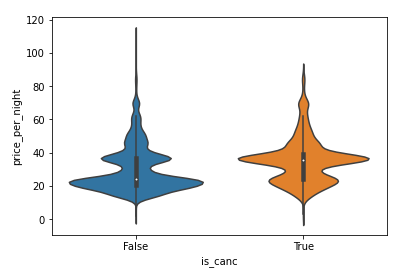
\includegraphics[width=10cm]{figures/price_per_night.png}
 \caption{A violin plot illustrating the distribution of price per night for student accommodation bookings, comparing cancelled and non cancelled bookings. False (blue) represents non-cancelled and True (orange)  represents cancelled bookings.}
\end{figure}
  
 Figure 4.1 compares the distribution of price per night when looking at bookings that cancelled to ones that did not. The mean price per night for bookings that cancelled is £35 per night compared to £29 per night for not cancelled bookings. This difference in price distribution when comparing cancelled to non cancelled bookings suggests price per night is an important feature for classification. 

 
 \begin{figure}[H]
 \centering
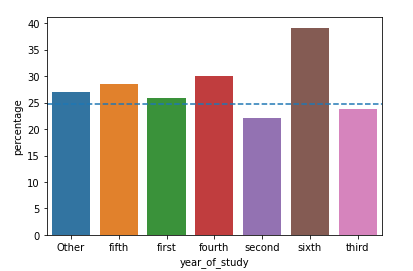
\includegraphics[width=10cm]{figures/yos.png}
 \caption{A bar graph showing the relative frequencies of the unique values as a percentage of booking cancellations in the student accommodation industry. Data is plotted by degree year of study with the blue horizontal line representing the mean cancellations.}
\end{figure}
  
Figure 4.2 shows percentage of booking cancellations grouped by academic year of study. This shows sixth years as having 40 percent cancellations, this may be due to the fact they are more likely to decide to live in private accommodation but it is unlikely this accounts for them being almost twice as likely to cancel than the average. The Other category is also an outlier here with a 27 percent chance of cancelling, more research would be needed to understand exactly why customers who do not enter a year of study are more likely to cancel but it is clear from this figure that year of study will be a good indicator of cancellations.

\vspace{5mm}
  
  \begin{figure}[H]
 \centering
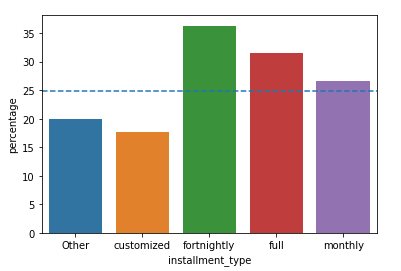
\includegraphics[width=7cm]{figures/instalment_type.png}
 \caption{A bar graph illustrating the relative frequencies of the unique values as a percentage of booking cancellations for payment instalment type in the student accommodation industry booking dataset. The blue horizontal line indicates the mean cancellation. Full payment plans represent the student playing all at once, monthly and fortnightly payment plans indicate the students paying at regular time intervals and customised payments allow the student to create their own plan. }
\end{figure}
  
  
 Figure 4.3 shows the weighted average of cancellations looking at the selected instalment type. Instalment type is the payment plan the student selected, we can see that students who selected the fortnightly plan are 10 percent more likely to cancel than the average, and students who opted for the customized instalment plan are 7 percent less likely to cancel. This may be a good predictor of cancellations.
  
  
   \begin{figure}[H]
 \centering
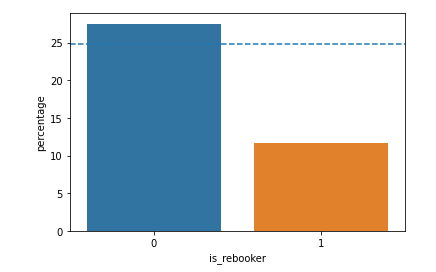
\includegraphics[width=10cm]{figures/is_rebooker.png}
 \caption{A bar graph illustrating the relative frequencies of the unique values as a percentage of booking cancellations for a rebooker, someone who has booked before. 0 (blue) represents a individual who has not booked before, 1(orange) represents someone who has.}
\end{figure}
  
Figure 4.4 shows the comparison of cancellations between students who are rebookers (have booked before) and those who are not. We can see that students who have not booked previously are 16 percent more likely to cancel their bookings. This is another good predictor of cancellations.  
 
 \section{Original Model - XGBoost}

\begin{figure}[H]
 \centering
  \begin{subfigure}{A\textwidth}
    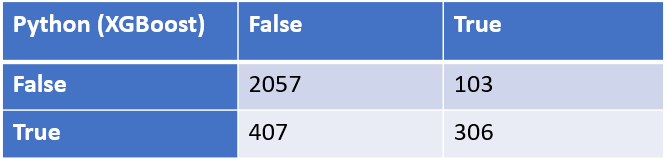
\includegraphics[width=10cm]{figures/python_xgboost.png}
  \end{subfigure}

  \centering
  \begin{subfigure}{B\textwidth}
    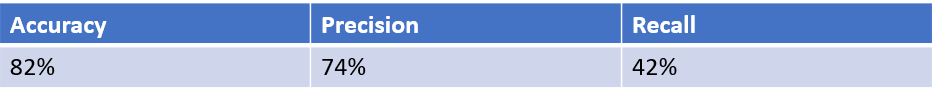
\includegraphics[width=10cm]{figures/python_recall}
    \caption{\textbf{These tables illustrate the original XGBoosts methods results.}\vspace{2mm} \\ A = The confusion matrix produced from the student accommodation booking data. False False: a non cancelled booking correctly predicted, False True: booking predicted as not cancelled but actually cancelled. True True: predicted as cancelled and actually cancelled and True False: predicted as cancelled but not actually cancelled.\vspace{2mm} \\B = A table illustrating the accuracy, precision and recall of the XGBoost method as a percentage.} \label{fig:1b}
  \end{subfigure}
\end{figure}

The confusion matrix in Figure 4.5 is a table that displays the performance of a classification model on a set of test data where the true values are known. The 4 sections that make up a confusion matrix are, true positives (TP) these are bookings that the model predicted as cancelled and are actually cancelled. True negatives (TN) these are bookings predicted correctly as not cancelled. False positives (FP) are bookings that the model predicted as cancelled but did not and False negatives (FN) these are bookings the model predicted as not cancelled but did cancel. TP is the most important because this is where the model has predicted a booking as going  to cancel and has actually cancelled which is the objective of this research.

\vspace{5mm}

The accuracy of a classification model is (TP+TN)/total. This is the number of bookings accurately classified as either cancelled or not cancelled. In this case it is more valuable to classify TP than TN since cancelled bookings are the focus of this research. Recall is TP / (TP + FN), this is the proportion of actual positive values predicted correctly.

\vspace{5mm}

 \begin{figure}[H]
 \centering
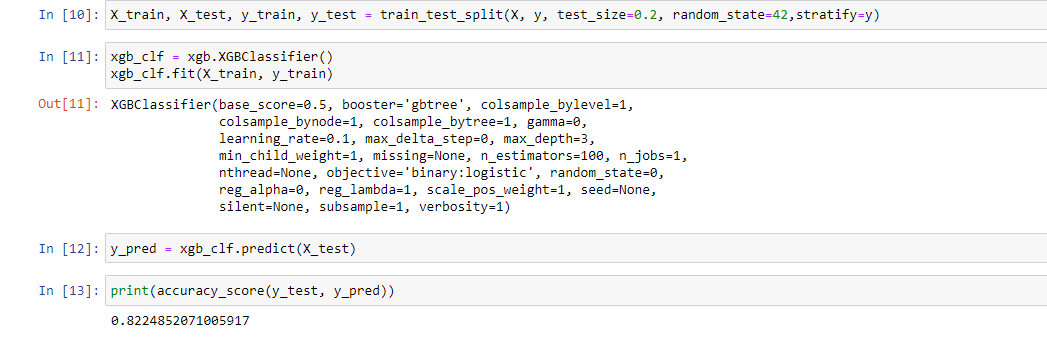
\includegraphics[width=10cm]{figures/xg_boost_code.png}
 \caption{The original code used for running the XGBoost model. A test size of 20 percent was used and the XGBoost classifier was created and then fit to the training data. Prediction shows 82 percent accuracy overall on the test data.}
\end{figure}

The original methodology included using Python to run XGBoost, Figure 4.6 shows a snippet of the code used to train the model with a train test split set to 20 percent. The model was created on the test data and the accuracy score was calculated. The model was run using the default hyper parameters, in sklearn. Initially, the accuracy score of 82 percent appeared to solve the problem specification. However, the confusion matrix shown in Figure 4.6 identified that there is a large number of false positive predictions compared with the number of true positive predictions, showing that the models recall is low compared to the accuracy. As recall identifies the number of true positives, correct cancellations, a low recall score is undesirable.


After running this model and identifying poor recall, an alternative model and Hyperparameter optimization needed to be identified to produce increase recall. Using Auto ML, different algorithms were tested to enable the best algorithm to be identified. 

\section{Auto ML}

Since Auto ML is automated, it allows for more effective testing and evaluation of different models and hyper parameter combinations. This addresses the previous issue of not knowing which model and hyper parameter combination to use in order to solve this problem.

 \begin{figure}[H]
 \centering
  \begin{subfigure}{A\textwidth}
    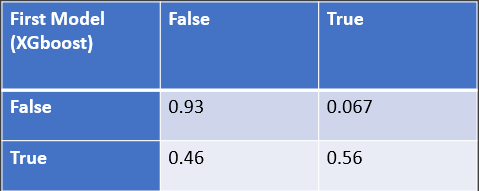
\includegraphics[width=10cm]{figures/xgboost_confusion_matrix.png}
  \end{subfigure}

  \centering
  \begin{subfigure}{B\textwidth}
    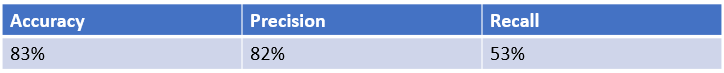
\includegraphics[width=10cm]{figures/original_results.png}
    \caption{\textbf{These tables illustrate the first Auto ML model results.}\vspace{2mm} \\ A= The confusion matrix produced from the student accommodation booking data presenting as normalized. False False: a non cancelled booking correctly predicted, False True: booking predicted as not cancelled but actually cancelled. True True: predicted as cancelled and actually cancelled and True False: predicted as cancelled but not actually cancelled. \vspace{2mm} \\B= A table illustrating the accuracy, precision and recall of the first Auto ML method.} \label{fig:1b}
  \end{subfigure}
\end{figure}

Figure 4.7 shows  0.93TF 0.56TP gives an overall accuracy of 0.83, this is inline with the results of running XGBoost manually outside of Auto ML. Figure 4.7 also shows only 53 percent of true positive values are identified correctly in the first run of Auto ML. This is only slightly better than the results of the original XGBoost model, with a high accuracy and low recall the original problem statement has not been solved. 

\section{Auto ML- Stack Ensemble}
Stack Ensemble learns how to merge predictions using a meta-learning algorithm from two or more base machine learning algorithms. The benefit of the stack is the fact that a variety of high performance models incorporate the capabilities to predict that any single model in the ensemble is superior to one classification. This is made up from 2 or more base models and a meta model that combines the predictions of the base models.

\vspace{5mm}

Knowing that recall should be the primary metric to target and not accuracy, using Auto ML, the target metric was changed to recall. Figure 3.5 shows the settings applied with the new primary metric being normalized macro recall. Setting the primary metric means Auto ML can optimise the model selection based on recall.

 \begin{figure}[H]
 \centering
\includegraphics[width=10cm]{figures/auto_ml_final_models.png}
 \caption{A table outlining the different algorithms used for the final run of Auto ML and the scaler used on the student accommodation booking data. Models were ranked by their recall (norm macro recall).}
\end{figure}

During this run Auto ML was used to evaluate and compare multiple different algorithms knowing that the algorithm with the best recall needed to be used, Auto ML was run again keeping all other values the same, and only changing the primary metric. Auto ML performs 15 different cross-validations on the data set, ranking them by the target attribute, recall (Figure 4.8). The same dataset and train test split were used,  meaning the model evaluates and ranks the results differently.

\begin{figure}[H]
 \centering
  \begin{subfigure}{A\textwidth}
    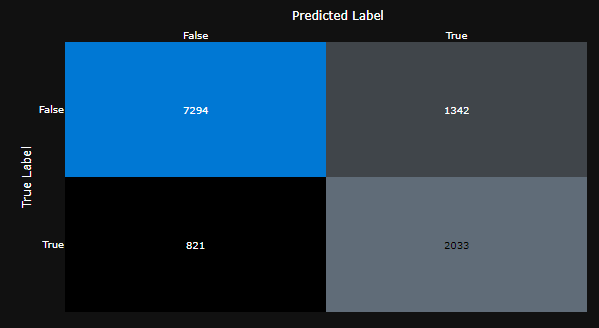
\includegraphics[width=10cm]{figures/azure_ml_confusion_matrix.png}
  \end{subfigure}

  \centering
  \begin{subfigure}{B\textwidth}
    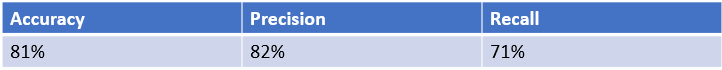
\includegraphics[width=10cm]{figures/final_recall.png}
    \caption{\textbf{These tables illustrate the final Auto ML, Stack Ensemble model results.}\vspace{2mm} \\ A = The confusion matrix produced from the student accommodation booking data presented as normalized. False False: a non cancelled booking correctly predicted, False True: booking predicted as not cancelled but actually cancelled. True True: predicted as cancelled and actually cancelled and True False: predicted as cancelled but not actually cancelled. \vspace{2mm} \\B = A table illustrating the accuracy, precision and recall of the final Auto ML, Stack Ensemble method.} \label{fig:1b}
  \end{subfigure}
\end{figure}

The confusion matrix in Figure 4.9 shows a significant improvement in recall when compared to the confusion matrix in Figure 4.6. This outlines the benefit of using the Stack Ensemble algorithm compared to XGBoost. 

\vspace{5mm}

In comparison to Figure 4.6, the final confusion matrix has a lower overall accuracy score but a higher recall score. The recall is a representation of the true predicted cancellations, a higher recall score is more desirable. The final model had a recall score of 71 percent (Figure 4.9) which is 18 percent higher than the original model. 

\begin{figure}[H]
 \centering
 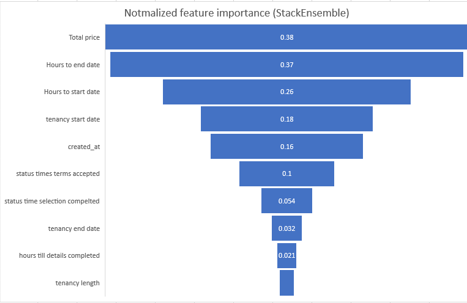
\includegraphics[width=10cm]{figures/feature_importance.png}
 \caption{A bar graph showing the feature importance of the final Auto ML model, ordered from high to low. }
\end{figure}

Based on the results from the feature importance graph in Figure 4.10, the main dependent feature on cancellations was total price, this was consistent with the feature exploration graph in Figure 4.1 which indicated price per night to be the most important feature. However, the rest of the features indicated in the exploratory data analysis were not present in the feature importance graph in Figure 4.10. The majority of the features in the feature importance graph were based on numerical data, such as hours to start or end date. 


\begin{figure}[H]
 \centering
 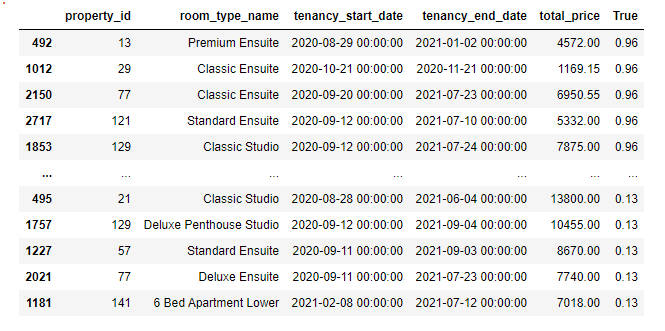
\includegraphics[width=10cm]{figures/canc_prob.png}
 \caption{A table of prediction probabilities, ranking each of the bookings made by their chance of cancellation, using the Stack Ensemble model on the student accommodation data. Property ID represents the unique property. True represents the chance of the booking being cancelled.}
\end{figure}
All of the bookings in the test data are ranked between 0 and 1, a booking over 0.5 gets classified as cancelled. The prediction probability was calculated using the Stack Ensemble model and is able to rank bookings made by the chance of them being cancelled.



